\section{Problem definition}

We commence with a training dataset comprising:
\begin{align*}
    &\left\{u(1),u(2),\cdots,u(N)\right\} \\
    &\left\{y(1),y(2),\cdots,y(N)\right\} \\
    &\left\{x(1),x(2),\cdots,x(N)\right\}
\end{align*}
In this methodology, during the design and training phase, complete state measurements are required. 
Therefore, initially, more sensors than the final system configuration are necessary.
Now, the goal is to identify a system with the given input-output relationship.

\paragraph*{Model}
We seek a model with the depicted architecture:
\begin{figure}[H]
    \centering
    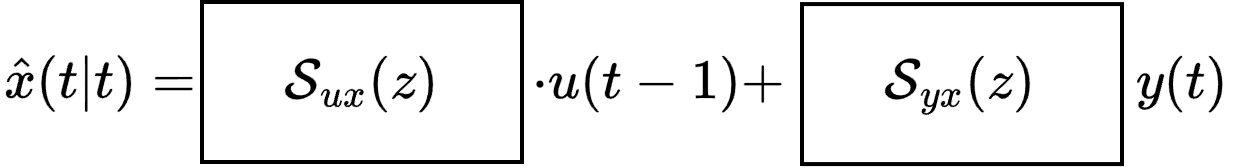
\includegraphics[width=0.75\linewidth]{images/arch.png}
\end{figure}
That is,
\[\hat{x}(t)=\mathcal{S}_{ux}(\mathcal{Z},\vartheta)u(t-1)+\mathcal{S}_{yx}(\mathcal{Z},\vartheta)y(t)\]
Here, the transfer functions $\mathcal{S}_{ux}$ and $\mathcal{S}_{yx}$ need to be determined.
To achieve this, we can employ the standard parametric approach:
\[J_N(\vartheta)=\dfrac{1}{N}\sum_{t=1}^{N}\left(x(t)-\left(\mathcal{S}_{ux}(\mathcal{Z},\vartheta)u(t-1)+\mathcal{S}_{yx}(\mathcal{Z},\vartheta)y(t)\right)\right)^2\]
The optimization step involves:
\[\hat{\vartheta}_N=\argmin_{\vartheta}J_N(\vartheta)\]
Resulting in:
\[\hat{x}(t)=\mathcal{S}_{ux}(\mathcal{Z},\hat{\vartheta}_N)u(t-1)+\mathcal{S}_{yx}(\mathcal{Z},\hat{\vartheta}_N)y(t)\]
This represents the estimation of the desired software sensor.

\paragraph*{Remarks}
Once the software sensing algorithm has been devised, physical state sensors can be removed.
The above approach can also be implemented using alternative system identification methods such as 4SID.